\chapter{Pulse Shape Discrimination}
\label{chapter:PSD}

\section{Traditional \ac{PSD}}
\label{sec:trditionalPSD}


\subsection{Amplitude/Energy cut}
\begin{figure}[H]
    \centering
    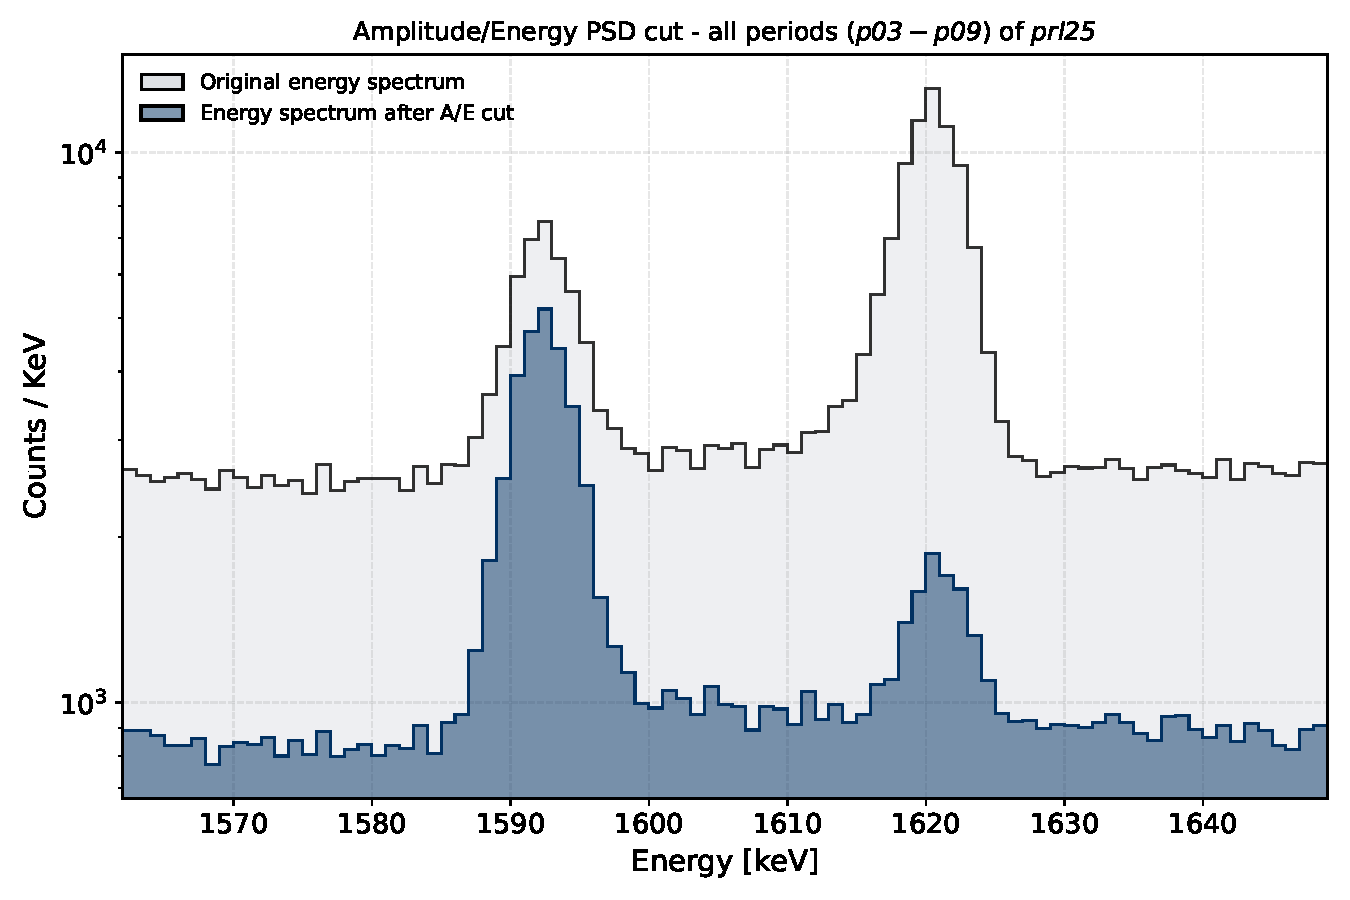
\includegraphics[width=0.7\textwidth]{plots/energy_specrum-prl25-AoE_cut.pdf}
    \caption{Windowed energy spectrum before (gray) and after (blue) the A/E cut. 90\% of the \ac{SSE} survives while almost all the \ac{MSE} are cut away.}
    \label{fig:dAoE_prl25}
\end{figure}